\documentclass[border=5pt]{standalone}
\usepackage[T1]{fontenc}
\usepackage[utf8]{inputenc}
\usepackage{amsmath}
\usepackage{graphicx}
\usepackage{tikz}
\usetikzlibrary{positioning,arrows.meta,calc}
\begin{document}
\resizebox{150mm}{!}{%
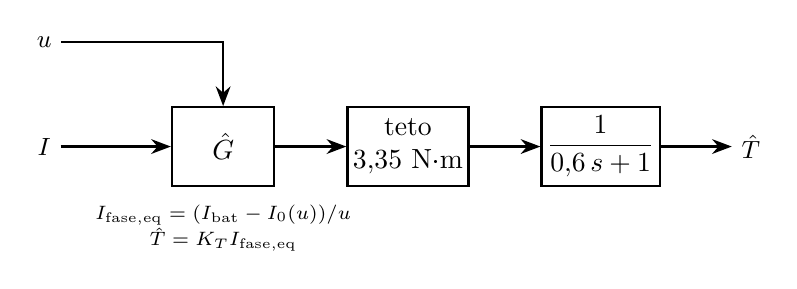
\begin{tikzpicture}[
  block/.style={draw=black, thick, minimum height=10mm, minimum width=13mm, inner sep=2pt},
  sign/.style={font=\itshape\small},
  arr/.style={-{Stealth[length=2.5mm]}, thick},
  node distance=8mm and 9mm,
]
\node[sign] (I) {$I$};
\node[sign, above=9mm of I] (u) {$u$};
\node[block, right=14mm of I] (G) {$\hat{G}$};
\node[font=\scriptsize, below=1mm of G, align=center]
  {$I_{\mathrm{fase,eq}} = (I_{\mathrm{bat}} - I_0(u))/u$\\
   $\hat{T} = K_T I_{\mathrm{fase,eq}}$};
\node[block, right=of G, align=center] (teto) {teto\\ $3{,}35$ N·m};
\node[block, right=of teto] (filtro) {$\dfrac{1}{0{,}6\,s+1}$};
\node[sign, right=of filtro] (That) {$\hat{T}$};

\draw[arr] (I) -- (G);
\draw[arr] (u) -| (G);
\draw[arr] (G) -- (teto);
\draw[arr] (teto) -- (filtro);
\draw[arr] (filtro) -- (That);
\end{tikzpicture}%
}
\end{document}
